%
% This is the LaTeX template file for lecture notes for EE 382C/EE 361C.
%
% To familiarize yourself with this template, the body contains
% some examples of its use.  Look them over.  Then you can
% run LaTeX on this file.  After you have LaTeXed this file then
% you can look over the result either by printing it out with
% dvips or using xdvi.
%
% This template is based on the template for Prof. Sinclair's CS 270.

\documentclass[twoside]{article}
\usepackage{graphics}
\graphicspath{ {./images/} }
\usepackage{graphics, graphicx, wrapfig}
\setlength{\oddsidemargin}{0.25 in}
\setlength{\evensidemargin}{-0.25 in}
\setlength{\topmargin}{-0.6 in}
\setlength{\textwidth}{6.5 in}
\setlength{\textheight}{8.5 in}
\setlength{\headsep}{0.75 in}
\setlength{\parindent}{0 in}
\setlength{\parskip}{0.1 in}

%
% The following commands set up the lecnum (lecture number)
% counter and make various numbering schemes work relative
% to the lecture number.
%
\newcounter{lecnum}
\renewcommand{\thepage}{\thelecnum-\arabic{page}}
\renewcommand{\thesection}{\thelecnum.\arabic{section}}
\renewcommand{\theequation}{\thelecnum.\arabic{equation}}
\renewcommand{\thefigure}{\thelecnum.\arabic{figure}}
\renewcommand{\thetable}{\thelecnum.\arabic{table}}

%
% The following macro is used to generate the header.
%
\newcommand{\lecture}[4]{
   \pagestyle{myheadings}
   \thispagestyle{plain}
   \newpage
   \setcounter{lecnum}{#1}
   \setcounter{page}{1}
   \noindent
   \begin{center}
   \framebox{
      \vbox{\vspace{2mm}
    \hbox to 6.28in { {\bf EE 382V: Social Computing
                        \hfill Fall 2018} }
       \vspace{4mm}
       \hbox to 6.28in { {\Large \hfill Lecture #1: #2  \hfill} }
       \vspace{2mm}
       \hbox to 6.28in { {\it Lecturer: #3 \hfill Scribe: #4} }
      \vspace{2mm}}
   }
   \end{center}
   \markboth{Lecture #1: #2}{Lecture #1: #2}
   %{\bf Disclaimer}: {\it These notes have not been subjected to the
   %usual scrutiny reserved for formal publications.  They may be distributed
   %outside this class only with the permission of the Instructor.}
   \vspace*{4mm}
}

%
% Convention for citations is authors' initials followed by the year.
% For example, to cite a paper by Leighton and Maggs you would type
% \cite{LM89}, and to cite a paper by Strassen you would type \cite{S69}.
% (To avoid bibliography problems, for now we redefine the \cite command.)
% Also commands that create a suitable format for the reference list.
\renewcommand{\cite}[1]{[#1]}
\def\beginrefs{\begin{list}%
        {[\arabic{equation}]}{\usecounter{equation}
         \setlength{\leftmargin}{2.0truecm}\setlength{\labelsep}{0.4truecm}%
         \setlength{\labelwidth}{1.6truecm}}}
\def\endrefs{\end{list}}
\def\bibentry#1{\item[\hbox{[#1]}]}

%Use this command for a figure; it puts a figure in wherever you want it.
%usage: \fig{NUMBER}{SPACE-IN-INCHES}{CAPTION}
\newcommand{\fig}[3]{
      \vspace{#2}
      \begin{center}
      Figure \thelecnum.#1:~#3
      \end{center}
  }
% Use these for theorems, lemmas, proofs, etc.
\newtheorem{theorem}{Theorem}[lecnum]
\newtheorem{lemma}[theorem]{Lemma}
\newtheorem{proposition}[theorem]{Proposition}
\newtheorem{claim}[theorem]{Claim}
\newtheorem{corollary}[theorem]{Corollary}
\newtheorem{definition}[theorem]{Definition}
\newenvironment{proof}{{\bf Proof:}}{\hfill\rule{2mm}{2mm}}

% **** IF YOU WANT TO DEFINE ADDITIONAL MACROS FOR YOURSELF, PUT THEM HERE:

\begin{document}
%FILL IN THE RIGHT INFO.
%\lecture{**LECTURE-NUMBER**}{**DATE**}{**LECTURER**}{**SCRIBE**}
\lecture{1}{August 24}{Vijay Garg}{Jesus Valenzuela Ochoa}
%\footnotetext{These notes are partially based on those of Nigel Mansell.}

% **** YOUR NOTES GO HERE:

% Some general latex examples and examples making use of the
% macros follow.
%**** IN GENERAL, BE BRIEF. LONG SCRIBE NOTES, NO MATTER HOW WELL WRITTEN,
%**** ARE NEVER READ BY ANYBODY.
\section{\sc \textbf{Proof that no constricted set $\Rightarrow$ a Perfect Match ($PM$)} }

Use induction on n
$|A|=|B|= n$\\
\underline{\textbf{Base Case $n = 1$}}
\begin{center}
$a_1 \odot \leftrightarrow \odot b_1$, There is $PM$
\end{center}

\underline{\textbf{Induction Case}}\\
Assume that the theorem is true for all values above $|A| <n$

 \underline{\textbf{Case 1}}\\
$\exists S$ so that $ |S| \equiv |N(S)|$

\underline{\textbf{Case 2}}\\
$\forall S  : |S| < |N(S)|$

\subsection{Case 1.}
For a selected subset $S$ of vertices from set $A$, the size of a subset created with the neighbors of the elements of $S$, i.e. $N(S)$, equals the size of subset $S$.\\

\begin{minipage}{0.25\textwidth}
\begin{center}
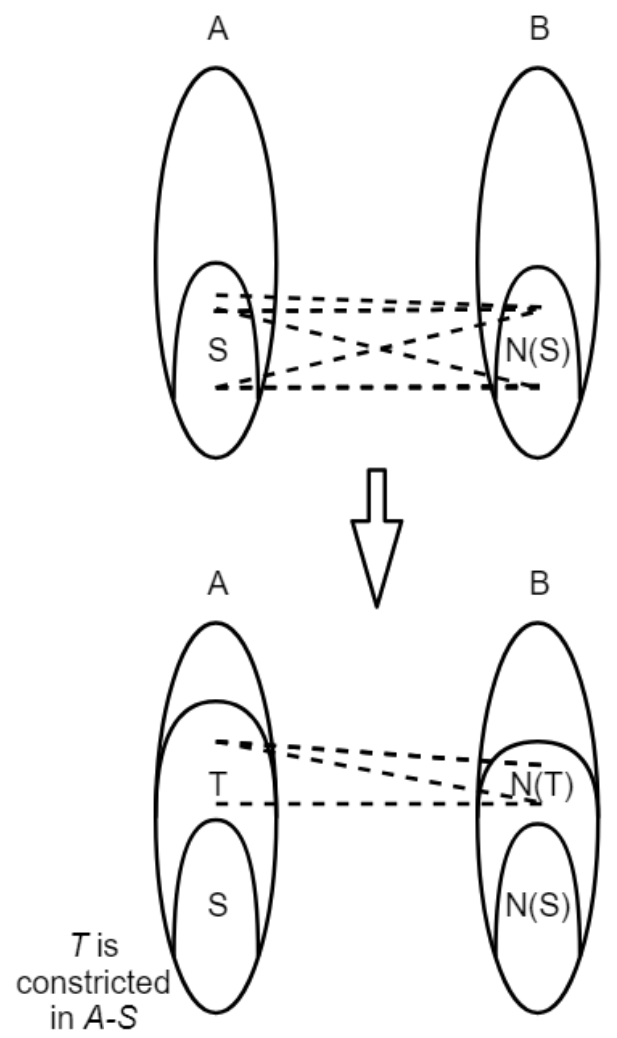
\includegraphics[scale=0.25]{split.png}
\fig{1}{0in}{Splitting sets.}
\end{center}
\end{minipage}
\begin{minipage}{0.75\textwidth}
It is needed to confirm that for the selected subsets $(S, N(S), E_s)$, the remaining subset $A-S$ does not have any constricted set when matched to subset $B-N(S)$.
\vspace{10mm}

This allows to iteratively break the problem into smaller parts, checking that remainder is not constricted after removing any given subset of A and its their neighbors.

\vspace{15mm}
If T is constricted in A-S(as shown in the lower section of Figure 1.1)\\
$\Rightarrow S \cup T$ is constricted in A $\Rightarrow$ \textbf{contradiction}
\vspace{20mm}

\end{minipage}

\newpage
\noindent \subsection{Case 2.}
For a selected subset $S$ of vertices from set $A$, the size of a subset created with the neighbors of the elements of $S$, i.e. $N(S)$, is less than the size of subset $S$.

Pick any vertex $a$ in $A$ and match to any vertex $b$ in $N(a)$, remove both $a$ and $b$ from the consideration.

- Verify that there is no constriction after removal.\\
- Now use induction as the set size has decreased.\\

In implementation, you want your algorithm to make matching maxim\textit{um} by the time it is maxim\textit{al}.

\section{Alternating Path}

An alternating path is one that alternates between matched and non-matched edges.
\begin{center}
\scalebox{.35}{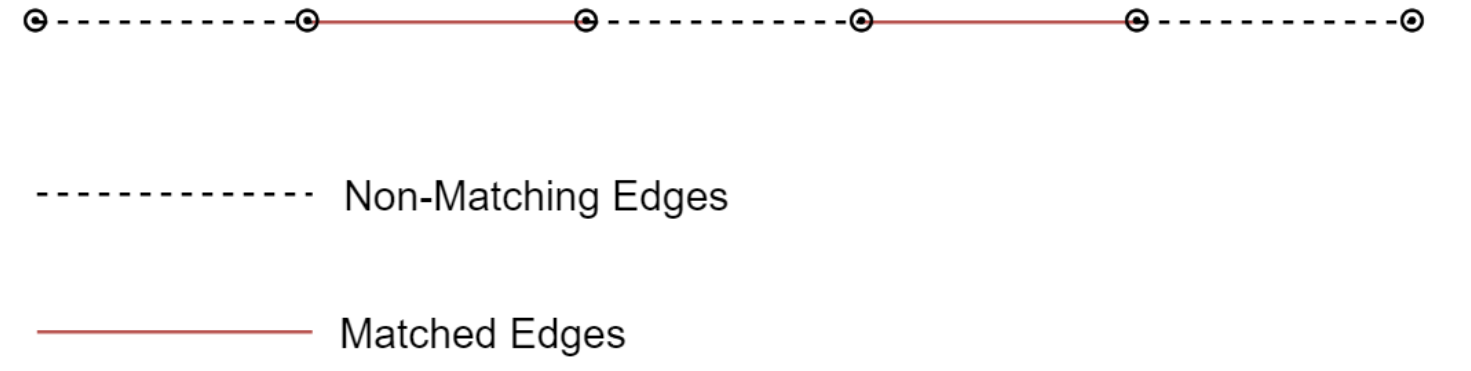
\includegraphics{altPath.png}}
\end{center}
\fig{2}{0in}{Alternating path.}

\subsection{Augmenting Path}
An \textit{augmenting path} is an alternating path starts with an exposed vertex in $A$ and ends with and exposed vertex in $B$. An \textbf{exposed vertex} is one that has only non-matching edges attached to it.

If an augmenting path is found, the size of the matching can be augmented (incremented by 1) by exchanging the matched edges for the non matched edges.\\

\begin{center}
\scalebox{.35}{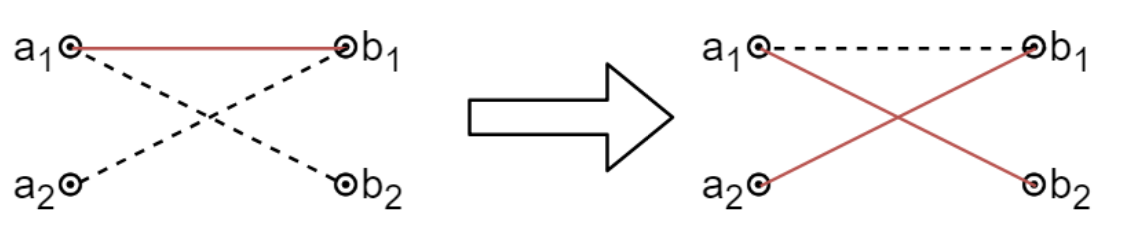
\includegraphics{invertColors.png}}\\
\end{center}
\fig{3}{0in}{Augmenting path edge exchange.}
All-edges start as unmatched. Consider using the B.F.S. algorithm to find a match. Always try to find an augmenting path.

\newpage
\underline{\textbf{B.F.S. Tree(with a twist)}}\\

\begin{minipage}{0.4\textwidth}
\scalebox{.25}{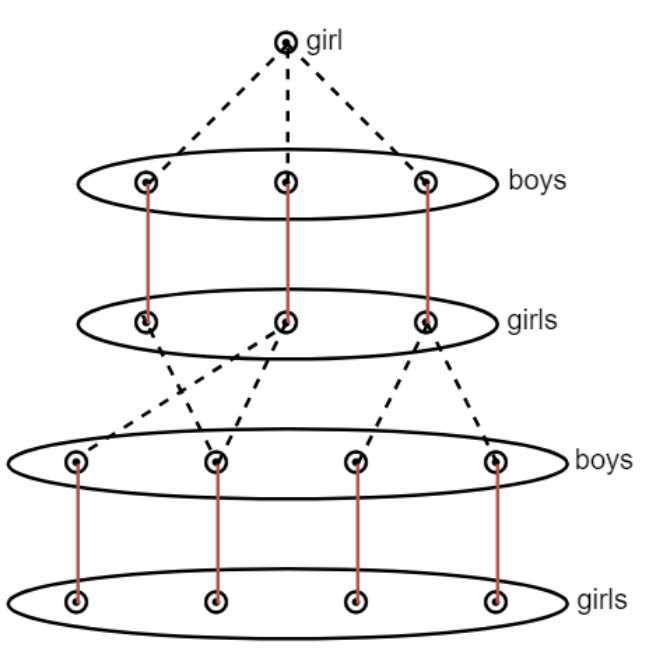
\includegraphics{BFSTree.png}}\\
\fig{4}{0in}{Example of a B.F.S.-Tree}
\end{minipage}
\begin{minipage}{0.6\textwidth}
This particular example has a constricted set, since there is one more girl than boys.

\vspace{13mm}
With B.F.S.-Tree construction, either an augmenting path is found or there is a constricted set. (By B.F.S.-Tree property).
\vspace{13mm}

\underline{\textbf{TIP}}

If there is no constricted set, then you know there is an augmenting path.\\
\end{minipage}



\begin{theorem}[Theorem]
A matching M is maxim\emph{um} if and only if there are no augmenting paths with respect to M.
\end{theorem}
\begin{proof}

- The existence of augmenting path indicates matching is not maxim\emph{um}, since matched and non-matching edges can be inverted, increasing matching size by 1.

- To prove that $M$ is not maximum $\Rightarrow \exists$  an augmenting path:\\

Let $M'$ be a maximum matching,
\begin{itemize}
\item Compute $ Q = M \bigtriangleup M' \leftarrow symmetrical$ \quad \quad \quad $(\bigtriangleup \equiv xor$ of $M$ and $M')$

 \quad \quad \quad \quad $M \bigtriangleup M' = (M'-M) \bigcup(M-M')$
\item Since $|M'| > |M|$, $Q $ has more edges from $M'$ than from $M$.
\item Each vertex is adjacent to at most one edge in $M \cap Q$ and at most one edges in $M' \cap Q$
\item $Q$ is composed of cycles(even number of edges) and paths(odd number of edges) that alternate between edges from $M$ and $M'$. Cycles will always be constructed by an even number of edges since we are working with bipartite graphs and a cycle with an odd number of edges would only be achievable by matching elements of the same set. Paths found must have more edges from $M'$ since its size is larger than that of $M$, hence representing the existence of an alternating augmenting path with reference to $M$, such as the one shown in Figure 1.5.
\end{itemize}
\begin{center}
\scalebox{.35}{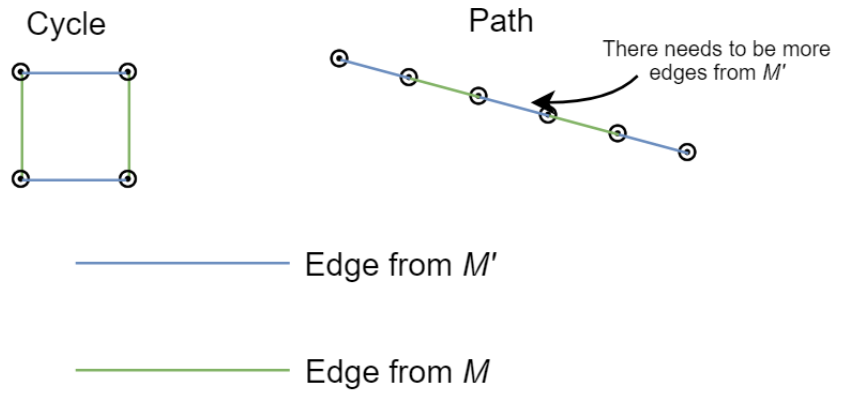
\includegraphics{cyclePath.png}}
\end{center}
\fig{5}{0in}{Cycle vs path construct}

\end{proof}
\section{Weak Duality}

Maximum matching problem with bipartite graphs:

\begin{center}
\scalebox{.25}{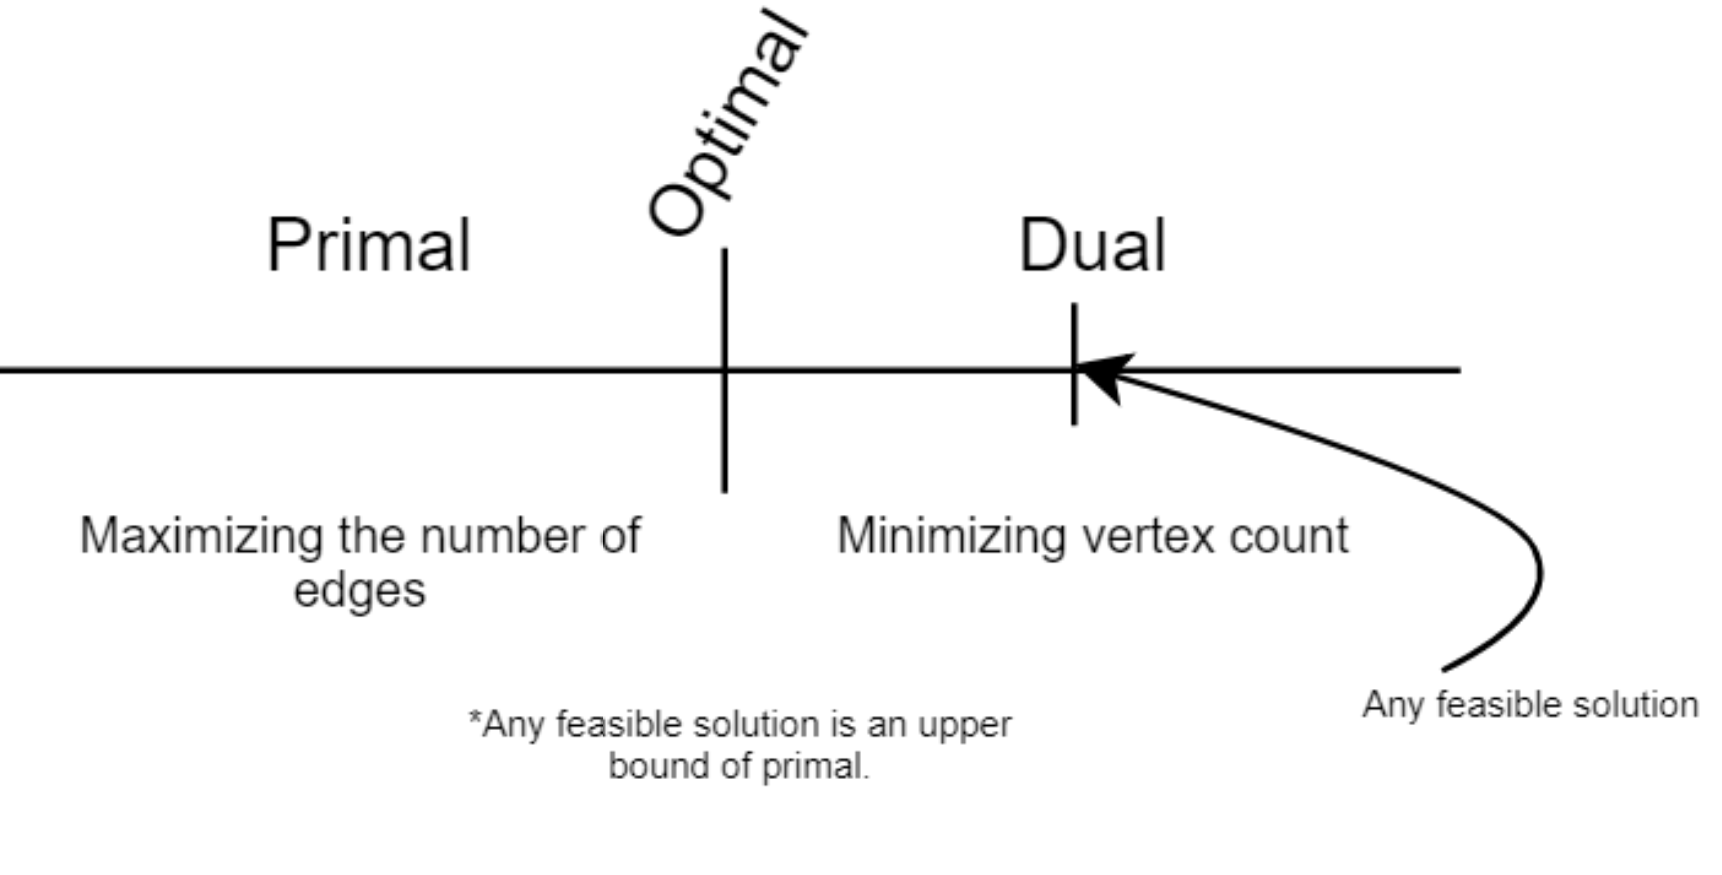
\includegraphics{weakDuality.png}}
\end{center}
\fig{6}{0in}{Weak duality in matching.}

Let $G$ be a bipartite graph, described as $G=(A,B,E)$. $X \subseteq A\cup B$ is a vertex cover of $G=(A,B,E)$ if every edge is adjacent to at least one vertex in X.\\
\begin{center}
\scalebox{.35}{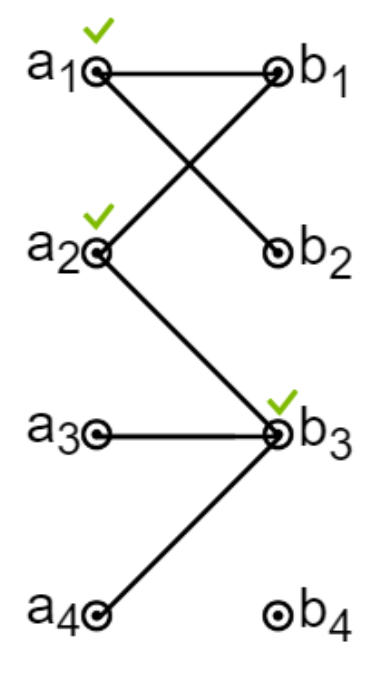
\includegraphics{vertexCover.png}}\\
\end{center}
\fig{7}{0in}{Example of a vertex cover. Analyzing what vertices combined are attached to all edges, we can establish $X=(a_1, a_2, b_3)$ for a cover of size 3.}

\begin{theorem}
Given any vertex cover $X$, and any matching $M$, $|M| \leq |X|$
\end{theorem}
\begin{proof}
Each element of $X$ can only have one match. All its other edges are removed once it matches.
\end{proof}
\begin{theorem}[K\"onig, Egerv\'ary Theorem]

For any bipartite graph, the maximum size of a matching equals the size of the minimum vertex cover.\\
\begin{center}
\scalebox{.35}{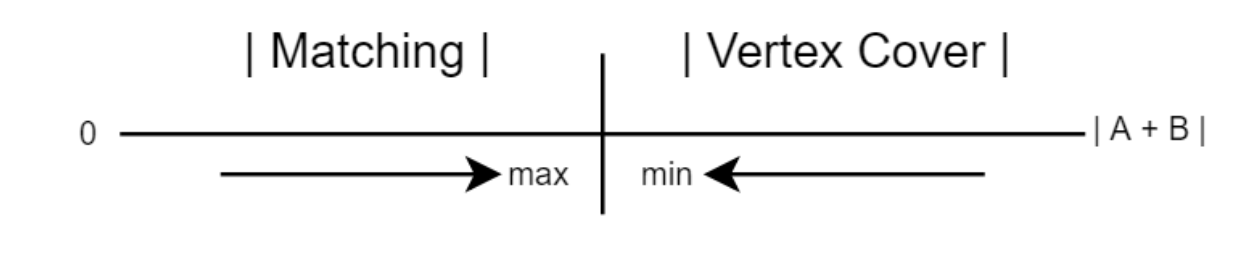
\includegraphics{minMax.png}}
\end{center}
\fig{8}{0in}{Min-Max theorem applied to weak duality in matching.}
\end{theorem}



\begin{minipage}{0.4\textwidth}
\scalebox{.35}{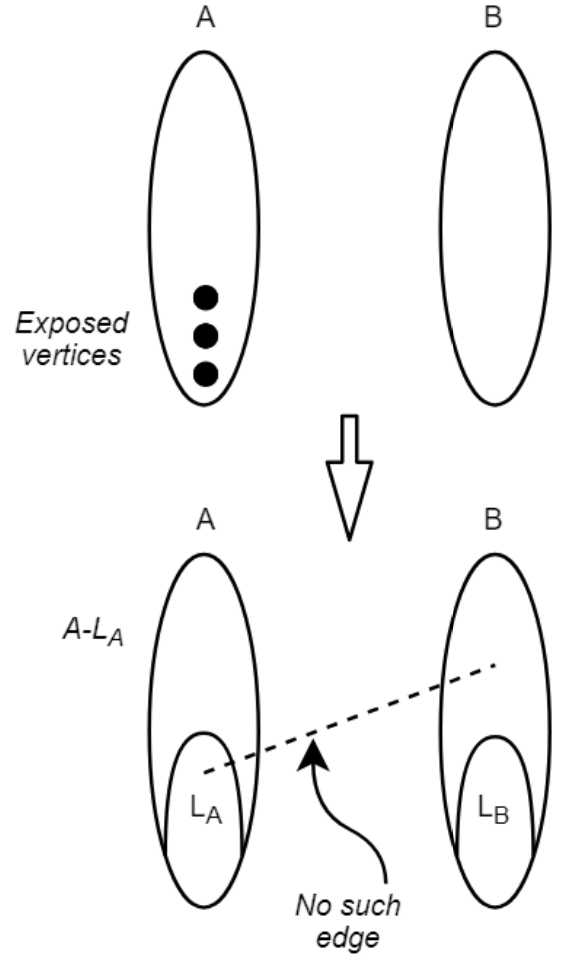
\includegraphics{KM.png}}\\
\fig{9}{0in}{Abstraction of sets into $L$. There may not be any edges between $L_A$ and $B - L$ as all the vertices in $L_A$ are either unmatched or have categorized edges they are connected to in $B$ into $L_B$, per $L$'s definition.}
\end{minipage}
\begin{minipage}{0.6\textwidth}
\textbf{Let}


$L$: Vertices that can be reached by B.F.S.-tree from an exposed vertex.\\

$M' : $ maximum matching of a bipartite graph.\\

$C' = (A-L_A)\cup L_B $\\

$L = L_A \cup L_B$\\
$L_A = A \cap L$\\
$L_B = B \cap L$

\vspace{10mm}
\textbf{Claim}\\
\begin{itemize}
\item $C'$ is a vertex cover.\\
Every edge in a bipartite graph belongs to either an alternating path, which places its $b_x$ endpoint in $B \cap L$, or it has an $a_x$ endpoint in $A-L_A$. If said edge is matched but not in an alternating path, then its $a_x$ endpoint cannot be in an alternating path, since said path must have included the edge and thus belongs to $A-L_A$. If the edge is unmatched but not in an alternating path, then its $a_x$ endpoint cannot be in an alternating path, for such a path could be extended by adding the edge to it. In consequence, $C'$ forms a vertex cover.
\item $|C'| = |M'|$\\
Every vertex in $C'$ is an endpoint of a matched edge: every vertex in $A-L_A$ is matched because $L$ includes all unmatched $A$ vertices, and every vertex in $B \cap L$ must also be matched, for if there existed an alternating path to an unmatched vertex then changing the matching by removing the matched edges from this path and adding the unmatched edges in their place would increase the size of the matching. However, no matched edge can have both of its endpoints in $C'$. Thus, $C'$ is a vertex cover of size equal to $M'$, and must be a minimum vertex cover.
\end{itemize}


\end{minipage}

\end{document}